%%%%%%%%%% BEGIN PREAMBLE %%%%%%%%%%
\documentclass[11pt,oneside]{book}
%%%%% PACKAGES %%%%%
\usepackage[top=2.54cm, bottom=2.54cm, left=3cm, right=2cm]{geometry}
\usepackage{graphicx}
\usepackage{lipsum}
\usepackage{amsmath}
\usepackage{amssymb}
\usepackage[font={scriptsize}]{caption}
\usepackage{float} 
\usepackage{changepage}
\usepackage{titlesec}
\usepackage{caption}
\usepackage{minitoc}

% minitoc parameters

\setlength{\mtcindent}{24pt}
\renewcommand{\mtcoffset}{0pt}
\mtcsetoffset{minitoc}{0pt}
\setlength{\mtcskipamount}{\bigskipamount}

\setcounter{minitocdepth}{2}  
\renewcommand{\mtcfont}{\small\rmfamily\upshape\mdseries} 
\renewcommand{\mtcSfont}{\small\rmfamily\upshape\bfseries}
% Suppress (sub)section printing in main ToC
\setcounter{tocdepth}{0}

% Change title offset
\titleformat{\chapter}[display]
	{\normalfont\huge\bfseries}{\chaptertitlename\ \thechapter}{20pt}{\Huge}
\titlespacing*{\chapter}{-.5in}{.5pt}{40pt}

%%%%%%%%%% TITLE PAGE %%%%%%%%%
% Create the command for including the title page in the document
\newcommand*{\titleGM}{\begingroup 
	\hbox{ % Horizontal box
		\hspace*{0.2\textwidth} % Whitespace to the left of the title page
		\rule{1pt}{\textheight} % Vertical line
		\hspace*{0.05\textwidth} % Whitespace between the vertical line and title page text
		\parbox[b]{0.75\textwidth}{ % Paragraph box which restricts text to less than the width of the page
			
			{\noindent\Huge\bfseries University of Manchester \\[0.5\baselineskip] Undergraduate \\[0.5\baselineskip]Physics Notes}\\[2\baselineskip] % Title
			{\large \textit{Volume 2}}\\[4\baselineskip] % Tagline or further description
			{\Large \textsc{E. Broadberry, H. Lee Hughes, N. K. Sen}} % Author name
			
			\vspace{0.5\textheight} % Whitespace between the title block and the publisher
	}}
	\endgroup}

%%%%% CUSTOM ENVIRONMENTS %%%%%
% "Examples" environment
\newenvironment{examples}[1][] %DON'T DELETE THESE BRACKETS IT WILL BREAK SHIT
	{\refstepcounter{subsection}
		\par
		\noindent\rule[0.2ex]{\linewidth}{0.1cm}
		\begin{adjustwidth}{1cm}{1cm}
		\medskip
		\noindent \textbf{Examples~\thesubsection #1} \rmfamily}
	{\par
		\end{adjustwidth}
		\noindent\rule[0.2ex]{\linewidth}{0.1cm}
		\medskip}

% "cust_figure" environment
\newenvironment{custfigure}[1][] %DON'T DELETE THESE BRACKETS IT WILL BREAK SHIT
	{\par #1
		\noindent\rule[0.2ex]{\linewidth}{1pt}
		\begin{figure}[H]
		\centering
		\captionsetup{font=small}
		}
	{\end{figure}
		\noindent\rule[0.2ex]{\linewidth}{1pt}
		\medskip}


%%%%% END PREABMLE %%%%%%

\begin{document}
\pagestyle{empty} % Removes page numbers

\titleGM % This command includes the title page

\dominitoc 
\tableofcontents

\chapter{This is the chapter title}
\minitoc

\pagebreak
As you can see the chapter title is offset from the text, if you wish to change the margins at all before finalise the template just do that and then do a pull request.
%
\section{Equation formatting options}
Section heading is not offset, perhaps we could change that, it's up to you?
 There are several different options for equations, I think there are 3 major things to think about:
%
\begin{enumerate}
	\item Vectors
	\item alignment
	\item problems?
\end{enumerate}
%
\subsection{1 - Vectors}
We're going with the bold vectors, use mathbf{} but pmb for the grad operator.
%
$$\pmb{\nabla}\times\mathbf{E} = \mathbf{\dot{B}}$$%
\subsection{2 - alignment}
This is really concerning lots of equation in a row for a long derivation, i'll give 2 they can be used in different situations, it's up to you.
%
$$\frac{1}{2}mv^2=\frac{3}{2}K_BT + A - A$$
%
$$v^2=\frac{3K_BT}{m}$$
%
$$v=\sqrt{\frac{3K_BT}{m}}$$
%
In that example the equations are all aligned in the middle
%
\begin{align*}	
	\frac{1}{2}mv^2&=\frac{3}{2}K_BT + A - A\\
	v^2&=\frac{3K_BT}{m}\\
	v&=\sqrt{\frac{3K_BT}{m}}\\
\end{align*}
%
Now all the equations are aligned at the equals sign, there's arguments for both but generally I think the first one looks more natural but its up to you.
%
\subsection{3 - problems}
For problems and examples I want to copy the Griffiths book, I'll show below.\\
%
\begin{examples}
	\begin{enumerate}
	\item Using maths, complete the following
	\begin{enumerate}
		\item Derive time
		\item Show that the soul survives after death
	\end{enumerate}
	\item By considering the twin paradox show:
	\begin{enumerate}
		\item Special relativity is wrong
		\item Kill yourself
	\end{enumerate}
\end{enumerate}
\end{examples}
%
\begin{minipage}[t]{0.47\linewidth}
\begin{custfigure} 
	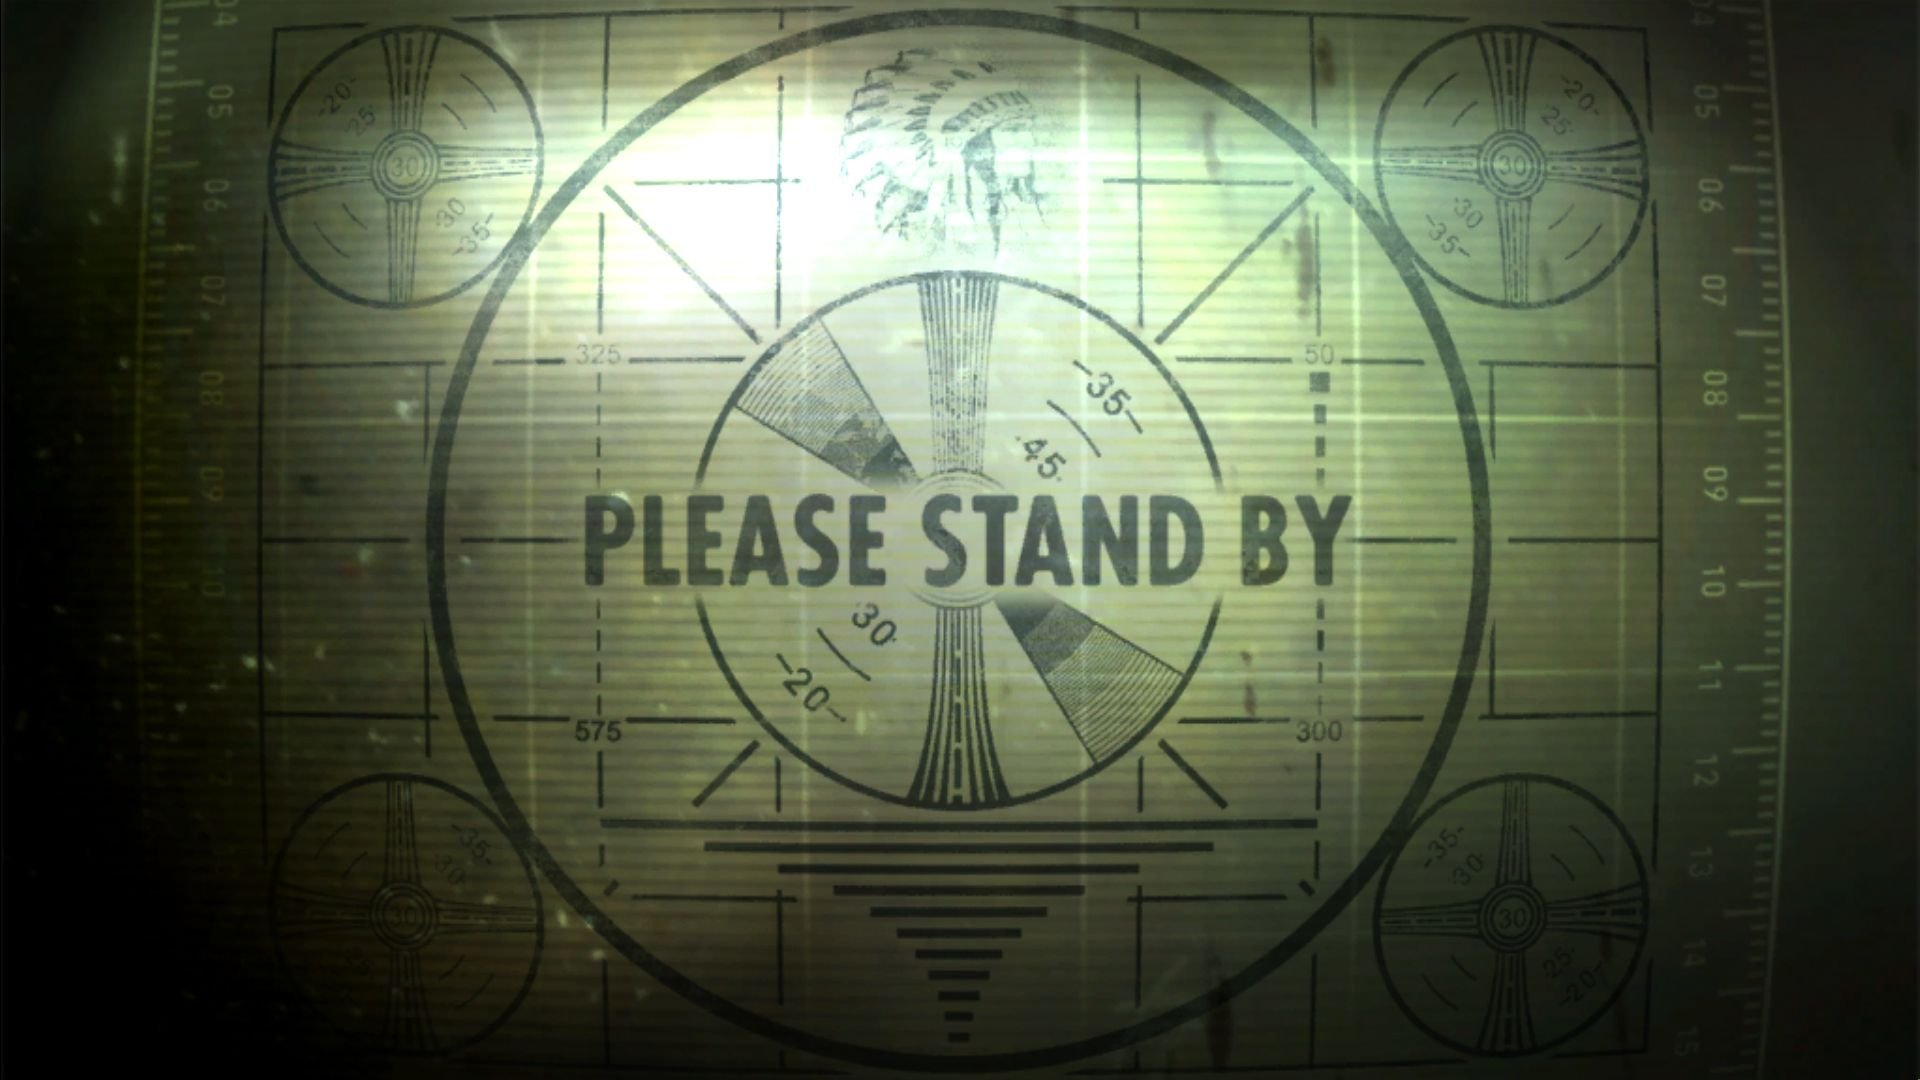
\includegraphics[width=\linewidth]{test-image}
	\caption{this is a caption}
\end{custfigure}
\end{minipage}
\hspace{0.6cm}
%
\begin{minipage}[t]{0.47\linewidth}
	\vspace{0.5cm}
	On the left is the custom figure environment in use, if you don't want the lines above and below then just insert a figure normally. This is an example of how to use minipages to put writing next to figures.
\end{minipage}
%
\section{test}
testy mctestest
\chapter{Test Chapter}
\minitoc
This is a test
\section{This is a section}
\begin{examples}
	\begin{enumerate}
		\item this is an example
		\item this is another example
	\end{enumerate}
\end{examples}

I have edited my test file.
\chapter{Test Chapter Part Duo}

Here is another test

\end{document}